%%% template.annotated.tex
%%%
%%% This LaTeX source document can be used as the basis for your technical
%%% paper or abstract. Unlike ``template.tex,'' this version of the source
%%% document contains documentation of each of the commands and definitions
%%% that should be used in the preparation of your formatted document.
%%% 
%%% The parameter given to the ``acmsiggraph'' LaTeX class in the 
%%% ``\documentclass'' command controls several features of the formatted 
%%% output: the presence or absence of hyperlinked icons just prior to the 
%%% first section of the paper, the amount of space left clear for the ACM
%%% copyright notice, the presence or absence of line numbers and submission
%%% ID, and the presence or absence of an appropriate ``preprint'' notice.
%%% 
%%% If you are preparing a paper for presentation in the Technical Papers
%%% program at one of our two annual flagship conferences, held in North 
%%% America (SIGGRAPH) or Asia (SIGGRAPH Asia), you should use ``tog''
%%% as the parameter.
%%%
%%% If you are preparing a paper for presentation at one of our sponsored
%%% events, including SIGGRAPH and SIGGRAPH Asia, but not in those events' 
%%% Technical Papers program, or a one- to four-page abstract, you should 
%%% use ``conference'' as the parameter.
%%% (Technical Briefs and Game Papers presented at our annual flagship 
%%% events fall into this category, as do papers accepted to other SIGGRAPH-
%%% sponsored events, such as I3D or ETRA or VRCAI, as do the one-page 
%%% abstracts which serve as the primary documentation for many of our 
%%% annual conference programs, including Posters, Talks, and Emerging 
%%% Technologies.)
%%%
%%% If you are preparing a version of your content for review, you should
%%% use ``review'' as the parameter. Line numbers will be added to your 
%%% paper, and the submission ID value will be printed across the top of 
%%% each page of your paper. (Use the submission ID as the parameter to the
%%% ``TOGonlineID'' command, below.)
%%%
%%% If you are preparing a preprint of your content, you should use
%%% ``preprint'' as the parameter. This is primarily for annual conference
%%% papers; a header reading ``To appear in ACM TOG X(Y)'' will appear on
%%% each page of the formatted output (where X is the volume and Y is the 
%%% number of the issue in which it will be published).

\documentclass[tog]{acmsiggraph}

%%% Definitions and commands that begin with ``\TOG'' are meant to be used
%%% in the preparation of papers to be presented in the Technical Papers
%%% program at one of our annual flagship events - SIGGRAPH and SIGGRAPH 
%%% Asia. You can safely ignore these definitions and commands if your 
%%% content is to be presented in some other venue.

%%% ``\TOGonlineid'' should be filled with the online ID value you received
%%% when you submitted your technical paper. It will be printed out if you 
%%% prepare a ``review'' version of your paper.

%\TOGonlineid{45678}

%%% Should your technical paper be accepted, you will be given three pieces
%%% of information: the volume and number of the issue of the ACM Transactions
%%% on Graphics journal in which your paper will be published, and the 
%%% ``article DOI'' value, which is unique to your paper and provides the 
%%% link to your paper's page in the ACM Digital Library. Fill in the 
%%% ``\TOGvolume,'' ``\TOGnumber,'' and ``\TOGarticleDOI'' definitions with
%%% the three pieces of information you receive.

%\TOGvolume{0}
%\TOGnumber{0}
%\TOGarticleDOI{1111111.2222222}

%%% By default, your technical paper will contain hyperlinked icons which 
%%% point to your paper's article page in the ACM Digital Library, and to 
%%% the paper itself in the ACM Digital Library. You may wish to add one 
%%% or more links to your own resources. If any of the following four 
%%% definitions have URLs in them, an appropriate hyperlinked icon will be
%%% added to the list. 

\TOGprojectURL{}
\TOGvideoURL{}
\TOGdataURL{}
\TOGcodeURL{}

%%% Define the title of your paper here. Use capital letters as appropriate.
%%% Setting the entire title in upper-case letters is not correct, nor is 
%%% capitalizing only the first letter of the title.

\title{A View from the Hill: Where Cross Reality Meets Virtual Worlds}

%%% Define the author list in the ``\author'' command. The ``\thanks'' 
%%% field can be used to define an e-mail address for the author.
%%% The ``\pdfauthor'' field should contain a comma-separated list of the
%%% authors of the paper, and is used, along with the title and keyword
%%% data, for PDF metadata. (To see this metadata, open the PDF in Adobe 
%%% Reader and select ``File > Properties > Description.''

\author{CJ Davies, Dr Alan Miller, Dr Colin Allison\\University of St Andrews}
\pdfauthor{CJ Davies, Dr Alan Miller, Dr Colin Allison}

%%% User-defined keywords.

\keywords{cross reality, head mounted display, indoor positioning}

%%% End of the document preamble, start of the document.

\begin{document}

%%% A ``teaser'' image appears below the title and affiliation and above
%%% the two-column body of the paper. This is optional, but if you wish
%%% to include such an image, the commented-out code, below, can be used
%%% as an example. Please note that the inclusion of a ``teaser'' image
%%% may move the copyright space to the bottom of the right-hand column
%%% on the first page of your formatted output. This is acceptable.

\teaser{
	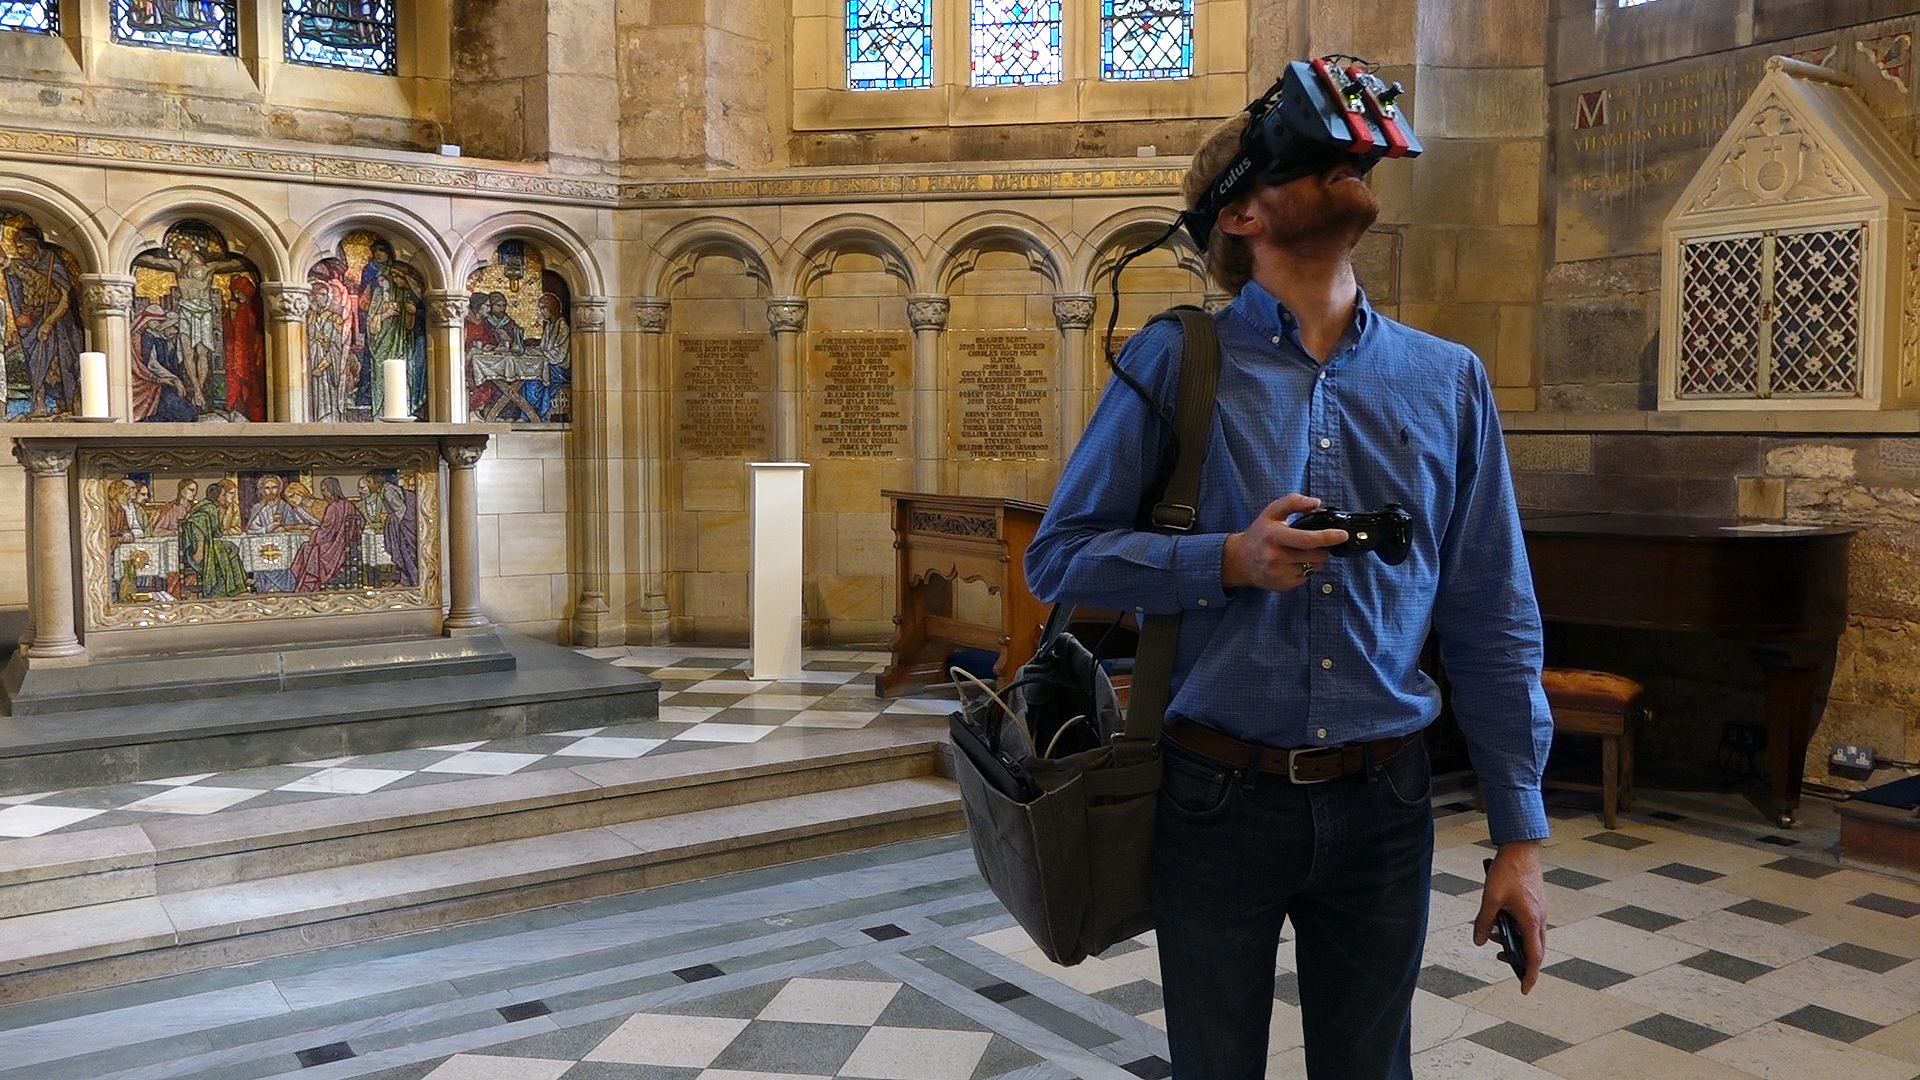
\includegraphics[height=2in]{images/teaser.png}
	\caption{A user study of the Mirrorshades platform under way in St Salvator's chapel, St Andrews.}
}

%%% The ``\maketitle'' command uses the author and title information 
%%% defined above, and prepares the formatted title.

\maketitle

%%% The ``abstract'' environment should contain the abstract for your
%%% content -- one to several paragraphs which describe the work.

\begin{abstract}
We present the cross reality~\cite{Lifton2007a} system `Mirrorshades', which enables a user to be present and aware of both a virtual reality environment and the real world at the same time. In so doing the challenge of the vacancy problem is addressed by lightening the cognitive load needed to switch between realities and to navigate the virtual environment. We present a case study in the context of a cultural heritage application wherein users are able to compare a reconstruction of an important 15th century chapel with its present day instantiation, whilst walking through them.

%Citations can be done this way~\cite{Jobs95} or this more concise 
%way~\shortcite{Jobs95}, depending upon the application.
\end{abstract}

%%% The ``CRCatlist'' environment defines one or more ACM ``Computing Review''
%%% (or ``CR'') categories, used for indexing your work. For more information
%%% on CR categories, please see http://www.acm.org/class/1998.

\begin{CRcatlist}
  \CRcat{I.3.7}{Computer Graphics}{Three-Dimensional Graphics and Realism}{Virtual reality};
\end{CRcatlist}

%%% The ``\keywordlist'' prints out the user-defined keywords.

\keywordlist

%%% If you are preparing a paper to be presented in the Technical Papers
%%% program at one of our annual flagship events (and, therefore, using 
%%% the ``tog'' parameter to the ``\documentclass'' command), the 
%%% ``\TOGlinkslist'' command prints out the list of hyperlinked icons.
%%% If you are using any other parameter to the ``\documentclass'' command
%%% this command does absolutely nothing.

\TOGlinkslist

%%% The ``\copyrightspace'' command will leave clear an amount of space
%%% at the bottom of the left-hand column on the first page of your paper,
%%% according to the parameter used in the ``\documentclass'' command.

\copyrightspace

%%% The first section of your paper. 

\section{Introduction and Implementation}

This research centers around the design, development and evaluation
of a hardware and software platform which allows its user to observe
and move around their Real World (RW) environment whilst wearing a wide field of view (FOV), stereoscopic 3D, Head Mounted
Display (HMD) which allows them to alternatively view an immersive Virtual Reality (VR) environment from the equivalent vantage
point. This is achieved by combining a head-tracked HMD, webcams, an indoor positioning system (IPS) and a 3D game engine, into
a mobile cross reality (XR) interface.

The novel aspect of this platform is the ability it imparts upon its user to transition between viewing equivalent vantage points in RW and VR environments. In order to achieve the highest quality of experience with this system, it is vital to determine how best to implement these transitions and as such multiple different transition styles have been implemented, including both those controlled by the user and those outwith their control.


\section{Case Study - Cultural Heritage}
Founded in 1450 but internally stripped of its medieval fittings during the Protestant Reformation (1517-1648), St Salvator's chapel in St Andrews looks markedly different today than it did upon its completion. An existing VR reconstruction of the chapel as it stood in 1450 and the marked differences between the internal appearance of the VR building and the current building make it an ideal candidate within the context of cultural heritage for a mobile XR system to be applied.

\section{Future Work}
User studies are under way in St Salvator's chapel to evaluate responses to the Mirrorshades platform in comparison to a traditional static VR experience and to assess reactions to and preferences toward different styles of transition between real and virtual environments.


%%% Please use the ``acmsiggraph'' BibTeX style to properly format your
%%% bibliography.

\bibliographystyle{acmsiggraph}
\bibliography{template}
\end{document}
